\documentclass[10pt]{article}
\usepackage[utf8]{inputenc}
\usepackage[T1]{fontenc}
\usepackage{amsmath}
\usepackage{amsfonts}
\usepackage{amssymb}
\usepackage[version=4]{mhchem}
\usepackage{stmaryrd}
\usepackage{bbold}
\usepackage{graphicx}
\usepackage[export]{adjustbox}
\graphicspath{ {./images/} }

\begin{document}
\section*{MATHEMATICS}
\section*{SECTION-A}
\begin{enumerate}
  \setcounter{enumi}{60}
  \item Let the function \(f(x)=2 x^{3}+(2 p-7) x^{2}+3(2 p-9) x-6\) have a maxima for some value of \(\mathrm{x}<0\) and a minima for some value of \(\mathrm{x}>0\). Then, the set of all values of \(p\) is\\
(1) \(\left(\frac{9}{2}, \infty\right)\)\\
(2) \(\left(0, \frac{9}{2}\right)\)\\
(3) \(\left(-\infty, \frac{9}{2}\right)\)\\
(4) \(\left(-\frac{9}{2}, \frac{9}{2}\right)\)
\end{enumerate}

Official Ans. by NTA (3)\\
Allen Ans. (3)\\
Sol. \(f(\mathrm{x})=2 \mathrm{x}^{3}+(2 \mathrm{p}-7) \mathrm{x}^{2}+3(2 \mathrm{p}-9) \mathrm{x}-6\)\\
\(f^{\prime}(\mathrm{x})=6 \mathrm{x}^{2}+2(2 \mathrm{p}-7) \mathrm{x}+3(2 \mathrm{p}-9)\)\\
\(f^{\prime}(0)<0\)\\
\(\therefore 3(2 p-9)<0\)

\[
\begin{aligned}
& \mathrm{p}<\frac{9}{2} \\
& \mathrm{p} \in\left(-\infty, \frac{9}{2}\right)
\end{aligned}
\]

\begin{enumerate}
  \setcounter{enumi}{61}
  \item Let \(z\) be a complex number such that \(\left|\frac{\mathrm{z}-2 \mathrm{i}}{\mathrm{z}+\mathrm{i}}\right|=2, \mathrm{z} \neq-\mathrm{i}\). Then z lies on the circle of radius 2 and centre\\
(1) \((2,0)\)\\
(2) \((0,0)\)\\
(3) \((0,2)\)\\
(4) \((0,-2)\)
\end{enumerate}

Official Ans. by NTA (4)\\
Allen Ans. (4)\\
Sol. \((z-2 i)(\bar{z}+2 i)=4(z+i)(\bar{z}-i)\)\\
\(z \bar{z}+4+2 i(z-\bar{z})=4(z \bar{z}+1+i(\bar{z}-z))\)\\
\(3 \mathrm{z} \overline{\mathrm{z}}-6 \mathrm{i}(\mathrm{z}-\overline{\mathrm{z}})=0\)\\
\(x^{2}+y^{2}-2 i(2 i y)=0\)\\
\(x^{2}+y^{2}+4 y=0\)

\section*{TEST PAPER WITH SOLUTION}
\begin{enumerate}
  \setcounter{enumi}{62}
  \item If the function\\
\(f(x)=\left\{\begin{array}{cl}(1+|\cos x|) \frac{\lambda}{|\cos x|}, & 0<x<\frac{\pi}{2} \\ \mu \quad & , x=\frac{\pi}{2} \quad \text { is continuous at } \\ e^{\frac{\cot 6 x}{\cot 4 x}} & , \frac{\pi}{2}<x<\pi\end{array}\right.\)\\
\(\mathrm{x}=\frac{\pi}{2}\), then \(9 \lambda+6 \log _{\mathrm{e}} \mu+\mu^{6}-\mathrm{e}^{6 \lambda}\) is equal to\\
(1) 11\\
(2) 8\\
(3) \(2 \mathrm{e}^{4}+8\)\\
(4) 10
\end{enumerate}

Official Ans. by NTA (4)\\
Allen Ans. BONUS\\
Sol. \(\Rightarrow \lim _{x \rightarrow \frac{\pi^{+}}{2}} e^{\frac{\cot 6 x}{\cot 4 x}}=\lim _{x \rightarrow \frac{\pi^{+}}{2}} e^{\frac{\sin 4 x \cdot \cos 6 x}{\sin 6 x \cdot \cos 4 x}}=e^{2 / 3}\)\\
\(\Rightarrow \lim _{x \rightarrow \frac{\pi^{-}}{2}}(1+|\cos x|)^{\left.\frac{\lambda}{\cos x} \right\rvert\,}=e^{\lambda}\)\\
\(\Rightarrow f(\pi / 2)=\mu\)\\
For continuous function \(\Rightarrow \mathrm{e}^{2 / 3}=\mathrm{e}^{\lambda}=\mu\)\\
\(\lambda=\frac{2}{3}, \mu=\mathrm{e}^{2 / 3}\)\\
Now, \(9 \lambda+6 \log _{\mathrm{e}} \mu+\mu^{6}-\mathrm{e}^{6 \lambda}=10\)\\
64. Let \(\mathrm{f}(\mathrm{x})=2 \mathrm{x}^{\mathrm{n}}+\lambda, \lambda \in \mathbb{R}, \mathrm{n} \in \mathbb{N}\), and \(\mathrm{f}(4)=133\), \(f(5)=255\). Then the sum of all the positive integer divisors of ( \(\mathrm{f}(3)-\mathrm{f}(2)\) ) is\\
(1) 61\\
(2) 60\\
(3) 58\\
(4) 59

Official Ans. by NTA (2)\\
Allen Ans. (2)\\
Sol. \(f(\mathrm{x})=2 \mathrm{x}^{\mathrm{n}}+\lambda\)\\
\(f(4)=133\)\\
\(f(5)=255\)\\
\(133=2 \times 4^{\mathrm{n}}+\lambda\)

\[
255=2 \times 5^{n}+\lambda
\]

(2) - (1)\\
\(122=2\left(5^{\mathrm{n}}-4^{\mathrm{n}}\right)\)\\
\(\Rightarrow 5^{n}-4^{n}=61\)\\
\(\therefore \mathrm{n}=3 \& \lambda=5\)\\
Now, \(f(3)-f(2)=2\left(3^{3}-2^{3}\right)=38\)\\
Number of Divisors is \(1,2,19,38\); \& their sum is 60\\
65. If the four points, whose position vectors are \(3 \hat{i}-4 \hat{j}+2 \hat{k}, \hat{i}+2 \hat{j}-\hat{k},-2 \hat{i}-\hat{j}+3 \hat{k}\) and \(5 \hat{i}-2 \alpha \hat{j}+4 \hat{k}\) are coplanar, then \(\alpha\) is equal to\\
(1) \(\frac{73}{17}\)\\
(2) \(-\frac{107}{17}\)\\
(3) \(-\frac{73}{17}\)\\
(4) \(\frac{107}{17}\)

Official Ans. by NTA (1)\\
Allen Ans. (1)\\
Sol. Let A : \((3,-4,2)\)\\
C : \((-2,-1,3)\)\\
B : \((1,2,-1)\)\\
D : \((5,-2 \alpha, 4)\)\\
\(\mathrm{A}, \mathrm{B}, \mathrm{C}, \mathrm{D}\) are coplanar points, then\\
\(\Rightarrow\left|\begin{array}{ccc}1-3 & 2+4 & -1-2 \\ -2-3 & -1+4 & 3-2 \\ 5-3 & -2 \alpha+4 & 4-2\end{array}\right|=0\)\\
\(\Rightarrow \alpha=\frac{73}{17}\)\\
66. Let \(\mathrm{A}=\left[\begin{array}{cc}\frac{1}{\sqrt{10}} & \frac{3}{\sqrt{10}} \\ \frac{-3}{\sqrt{10}} & \frac{1}{\sqrt{10}}\end{array}\right]\) and \(\mathrm{B}=\left[\begin{array}{cr}1 & -\mathrm{i} \\ 0 & 1\end{array}\right]\), where \(\mathrm{i}=\sqrt{-1}\). If \(\mathrm{M}=\mathrm{A}^{\mathrm{T}} \mathrm{BA}\), then the inverse of the matrix \(\mathrm{AM}^{2023} \mathrm{~A}^{\mathrm{T}}\) is\\
(1) \(\left[\begin{array}{cc}1 & -2023 i \\ 0 & 1\end{array}\right]\)\\
(2) \(\left[\begin{array}{ll}1 & 0 \\ -2023 \mathrm{i} & 1\end{array}\right]\)\\
(3) \(\left[\begin{array}{ll}1 & 0 \\ 2023 \mathrm{i} & 1\end{array}\right]\)\\
(4) \(\left[\begin{array}{cc}1 & 2023 \mathrm{i} \\ 0 & 1\end{array}\right]\)

Official Ans. by NTA (4)\\
Allen Ans. (4)

Sol. \(\quad \mathrm{AA}^{\mathrm{T}}=\left[\begin{array}{ll}\frac{1}{\sqrt{10}} & \frac{3}{\sqrt{10}} \\ \frac{-3}{\sqrt{10}} & \frac{1}{\sqrt{10}}\end{array}\right]\left[\begin{array}{ll}\frac{1}{\sqrt{10}} & \frac{-3}{\sqrt{10}} \\ \frac{3}{\sqrt{10}} & \frac{1}{\sqrt{10}}\end{array}\right]=\left[\begin{array}{ll}1 & 0 \\ 0 & 1\end{array}\right]\)\\
\(\mathrm{B}^{2}=\left[\begin{array}{cc}1 & -\mathrm{i} \\ 0 & 1\end{array}\right]\left[\begin{array}{cc}1 & -\mathrm{i} \\ 0 & 1\end{array}\right]=\left[\begin{array}{cc}1 & -2 \mathrm{i} \\ 0 & 1\end{array}\right]\)\\
\(\mathrm{B}^{3}=\left[\begin{array}{cc}1 & -3 \mathrm{i} \\ 0 & 1\end{array}\right]\)\\
\(\mathrm{B}^{2023}=\left[\begin{array}{cc}1 & -2023 \mathrm{i} \\ 0 & 1\end{array}\right]\)\\
\(\mathrm{M}=\mathrm{A}^{\mathrm{T}} \mathrm{BA}\)\\
\(\mathrm{M}^{2}=\mathrm{M} \cdot \mathrm{M}=\mathrm{A}^{\mathrm{T}} \mathrm{BA} \mathrm{A}^{\mathrm{T}} \mathrm{BA}=\mathrm{A}^{\mathrm{T}} \mathrm{B}^{2} \mathrm{~A}\)\\
\(M^{3}=M^{2} \cdot M=A^{T} B^{2} A A^{T} B A=A^{T} B^{3} A\)\\
.\\
.\\
.\\
\(\mathrm{M}^{2023}=\) \(\_\_\_\_\) \(\mathrm{A}^{\mathrm{T}} \mathrm{B}^{2023} \mathrm{~A}\)\\
\(\mathrm{AM}^{2023} \mathrm{~A}^{\mathrm{T}}=\mathrm{AA}^{\mathrm{T}} \mathrm{B}^{2023} \mathrm{AA}^{\mathrm{T}}=\mathrm{B}^{2023}\)\\
\(=\left[\begin{array}{cc}1 & -2023 \mathrm{i} \\ 0 & 1\end{array}\right]\)\\
Inverse of \(\left(\mathrm{AM}^{2023} \mathrm{~A}^{\mathrm{T}}\right)\) is \(\left[\begin{array}{cc}1 & 2023 \mathrm{i} \\ 0 & 1\end{array}\right]\)\\
67. Let \(\Delta, \nabla \in\{\wedge, \vee\}\) be such that \((\mathrm{p} \rightarrow \mathrm{q}) \Delta(\mathrm{p} \nabla \mathrm{q})\) is a tautology. Then\\
(1) \(\Delta=\wedge, \nabla=\vee\)\\
(2) \(\Delta=\vee, \nabla=\wedge\)\\
(3) \(\Delta=\vee, \nabla=\vee\)\\
(4) \(\Delta=\wedge, \nabla=\wedge\)

Official Ans. by NTA (3)\\
Allen Ans. (3)

Sol. Given \((\mathrm{p} \rightarrow \mathrm{q}) \Delta(\mathrm{p} \nabla \mathrm{q})\)\\
Option I \(\quad \Delta=\wedge, \nabla=\vee\)

\begin{center}
\begin{tabular}{|c|c|c|c|c|}
\hline
p & q & \((\mathrm{p} \rightarrow \mathrm{q})\) & \((\mathrm{p} \vee \mathrm{q})\) & \((\mathrm{p} \rightarrow \mathrm{q}) \wedge(\mathrm{p} \vee \mathrm{q})\) \\
\hline
T & T & T & T & T \\
\hline
T & F & F & T & F \\
\hline
F & T & T & T & T \\
\hline
F & F & T & F & F \\
\hline
\end{tabular}
\end{center}

Option \(2 \quad \Delta=\vee, \nabla=\wedge\)

\begin{center}
\begin{tabular}{|c|c|c|c|c|}
\hline
p & q & \((\mathrm{p} \rightarrow \mathrm{q})\) & \((\mathrm{p} \wedge \mathrm{q})\) & \((\mathrm{p} \rightarrow \mathrm{q}) \vee(\mathrm{p} \wedge \mathrm{q})\) \\
\hline
T & T & T & T & T \\
\hline
T & F & F & F & F \\
\hline
F & T & T & F & T \\
\hline
F & F & T & F & T \\
\hline
\end{tabular}
\end{center}

Option \(3 \quad \Delta=\vee, \nabla=\vee\)

\begin{center}
\begin{tabular}{|c|c|c|c|c|}
\hline
p & q & \((\mathrm{p} \rightarrow \mathrm{q})\) & \((\mathrm{p} \vee \mathrm{q})\) & \((\mathrm{p} \rightarrow \mathrm{q}) \vee(\mathrm{p} \wedge \mathrm{q})\) \\
\hline
T & T & T & T & T \\
\hline
T & F & F & T & T \\
\hline
F & T & T & T & T \\
\hline
F & F & T & F & T \\
\hline
\end{tabular}
\end{center}

Hence, it is tautology.\\
Option \(4 \Delta=\wedge, \nabla=\wedge\)

\begin{center}
\begin{tabular}{|c|c|c|c|c|}
\hline
p & q & \((\mathrm{p} \rightarrow \mathrm{q})\) & \((\mathrm{p} \wedge \mathrm{q})\) & \((\mathrm{p} \rightarrow \mathrm{q}) \wedge(\mathrm{p} \wedge \mathrm{q})\) \\
\hline
T & T & T & T & T \\
\hline
T & F & F & F & F \\
\hline
F & T & T & F & F \\
\hline
F & F & T & F & F \\
\hline
\end{tabular}
\end{center}

\begin{enumerate}
  \setcounter{enumi}{67}
  \item The number of numbers, strictly between 5000 and 10000 can be formed using the digits \(1,3,5,7,9\) without repetition, is\\
(1) 6\\
(2) 12\\
(3) 120\\
(4) 72
\end{enumerate}

Official Ans. by NTA (4)\\
Allen Ans. (4)\\
Sol. Numbers between 5000 \& 10000\\
Using digits 1, 3, 5, 7, 9\\
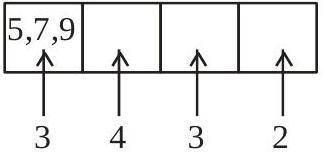
\includegraphics[max width=\textwidth, center]{2025_10_03_a6db97cda75dfa8b6db2g-03}

Total Numbers \(=3 \times 4 \times 3 \times 2=72\)\\
69. The number of functions \(f:\{1,2,3,4\} \rightarrow\{a \in \mathbb{Z}:|a| \leq 8\} \quad\) satisfying \(f(n)+ \frac{1}{n} f(n+1)=1, \forall n \in\{1,2,3\}\) is\\
(1) 3\\
(2) 4\\
(3) 1\\
(4) 2

Official Ans. by NTA (4)\\
Allen Ans. (4)\\
Sol. \(f:\{1,2,3,4\} \rightarrow\{\mathrm{a} \in \mathbb{Z}:|\mathrm{a}| \leq 8\}\)\\
\(f(\mathrm{n})+\frac{1}{\mathrm{n}} \mathrm{f}(\mathrm{n}+1)=1, \forall \mathrm{n} \in\{1,2,3\}\)\\
\(f(\mathrm{n}+1)\) must be divisible by n\\
\(f(4) \Rightarrow-6,-3,0,3,6\)\\
\(f(3) \Rightarrow-8,-6,-4,-2,0,2,4,6,8\)\\
\(f(2) \Rightarrow-8, \ldots \ldots \ldots \ldots \ldots, 8\)\\
\(f(1) \Rightarrow-8, \ldots \ldots \ldots \ldots \ldots, 8\)\\
\(\frac{\mathrm{f}(4)}{3}\) must be odd since \(f(3)\) should be even therefore 2 solution possible.

\begin{center}
\begin{tabular}{lclc}
\(f(4)\) & \(f(3)\) & \(f(2)\) & \(f(1)\) \\
-3 & 2 & 0 & 1 \\
3 & 0 & 1 & 0 \\
\end{tabular}
\end{center}

\begin{enumerate}
  \setcounter{enumi}{69}
  \item The equations of two sides of a variable triangle are \(\mathrm{x}=0\) and \(\mathrm{y}=3\), and its third side is a tangent to the parabola \(y^{2}=6 x\). The locus of its circumcentre is :\\
(1) \(4 y^{2}-18 y-3 x-18=0\)\\
(2) \(4 y^{2}+18 y+3 x+18=0\)\\
(3) \(4 y^{2}-18 y+3 x+18=0\)\\
(4) \(4 y^{2}-18 y-3 x+18=0\)
\end{enumerate}

Official Ans. by NTA (3)\\
Allen Ans. (3)\\
Sol. \(\quad y^{2}=6 x \quad \& y^{2}=4 a x\)\\
\(\Rightarrow 4 \mathrm{a}=6 \Rightarrow \mathrm{a}=\frac{3}{2}\)\\
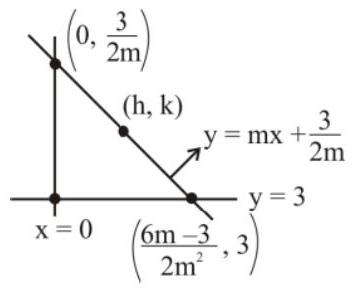
\includegraphics[max width=\textwidth, center]{2025_10_03_a6db97cda75dfa8b6db2g-03(1)}\\
\(\mathrm{y}=\mathrm{mx}+\frac{3}{2 \mathrm{~m}} ;(\mathrm{m} \neq 0)\)\\
\(h=\frac{6 m-3}{4 m^{2}}, k=\frac{6 m+3}{4 m}\), Now eliminating \(m\) and we get\\
\(\Rightarrow 3 \mathrm{~h}=2\left(-2 \mathrm{k}^{2}+9 \mathrm{k}-9\right)\)\\
\(\Rightarrow 4 \mathrm{y}^{2}-18 \mathrm{y}+3 \mathrm{x}+18=0\)\\
71. Let \(\mathrm{f}: \mathbb{R} \rightarrow \mathbb{R}\) be a function defined by \(\mathrm{f}(\mathrm{x})= \log _{\sqrt{m}}\{\sqrt{2}(\sin x-\cos x)+m-2\}\), for some \(m\), such that the range of f is \([0,2]\). Then the value of \(m\) is \(\_\_\_\_\)\\
(1) 5\\
(2) 3\\
(3) 2\\
(4) 4

Official Ans. by NTA (1)\\
Allen Ans. (1)\\
Sol. Since,\\
\(-\sqrt{2} \leq \sin x-\cos x \leq \sqrt{2}\)\\
\(\therefore-2 \leq \sqrt{2}(\sin x-\cos x) \leq 2\)\\
(Assume \(\sqrt{2}(\sin x-\cos x)=k\) )

\[
\begin{aligned}
& -2 \leq \mathrm{k} \leq 2 \quad \ldots(\mathrm{i}) \\
& f(\mathrm{x})=\log _{\sqrt{\mathrm{m}}}(\mathrm{k}+\mathrm{m}-2)
\end{aligned}
\]

Given,

\[
\begin{aligned}
& 0 \leq f(\mathrm{x}) \leq 2 \\
& 0 \leq \log _{\sqrt{\mathrm{m}}}(\mathrm{k}+\mathrm{m}-2) \leq 2 \\
& 1 \leq \mathrm{k}+\mathrm{m}-2 \leq \mathrm{m} \\
& -\mathrm{m}+3 \leq \mathrm{k} \leq 2 \ldots \text { (ii) }
\end{aligned}
\]

From eq. (i) \& (ii), we get \(-m+3=-2\)

\[
\Rightarrow \mathrm{m}=5
\]

\begin{enumerate}
  \setcounter{enumi}{71}
  \item Let \(\mathrm{A}, \mathrm{B}, \mathrm{C}\) be \(3 \times 3\) matrices such that A is symmetric and \(B\) and \(C\) are skew-symmetric.
\end{enumerate}

Consider the statements\\
(S1) \(\mathrm{A}^{13} \mathrm{~B}^{26}-\mathrm{B}^{26} \mathrm{~A}^{13}\) is symmetric\\
(S2) \(\mathrm{A}^{26} \mathrm{C}^{13}-\mathrm{C}^{13} \mathrm{~A}^{26}\) is symmetric\\
Then,\\
(1) Only S2 is true\\
(2) Only S1 is true\\
(3) Both S1 and S2 are false\\
(4) Both S1 and S2 are true

Official Ans. by NTA (1)\\
Allen Ans. (1)

Sol. Given, \(\mathrm{A}^{\mathrm{T}}=\mathrm{A}, \mathrm{B}^{\mathrm{T}}=-\mathrm{B}, \mathrm{C}^{\mathrm{T}}=-\mathrm{C}\)\\
Let \(M=A^{13} B^{26}-B^{26} A^{13}\)\\
Then, \(\mathrm{M}^{\mathrm{T}}=\left(\mathrm{A}^{13} \mathrm{~B}^{26}-\mathrm{B}^{26} \mathrm{~A}^{13}\right)^{\mathrm{T}}\)\\
\(=\left(\mathrm{A}^{13} \mathrm{~B}^{26}\right)^{\mathrm{T}}-\left(\mathrm{B}^{26} \mathrm{~A}^{13}\right)^{\mathrm{T}}\)\\
\(=\left(\mathrm{B}^{\mathrm{T}}\right)^{26}\left(\mathrm{~A}^{\mathrm{T}}\right)^{13}-\left(\mathrm{A}^{\mathrm{T}}\right)^{13}\left(\mathrm{~B}^{\mathrm{T}}\right)^{26}\)\\
\(=\mathrm{B}^{26} \mathrm{~A}^{13}-\mathrm{A}^{13} \mathrm{~B}^{26}=-\mathrm{M}\)\\
Hence, \(M\) is skew symmetric\\
Let, \(\mathrm{N}=\mathrm{A}^{26} \mathrm{C}^{13}-\mathrm{C}^{13} \mathrm{~A}^{26}\)\\
then, \(\mathrm{N}^{\mathrm{T}}=\left(\mathrm{A}^{26} \mathrm{C}^{13}\right)^{\mathrm{T}}-\left(\mathrm{C}^{13} \mathrm{~A}^{26}\right)^{\mathrm{T}}\)\\
\(=-(\mathrm{C})^{13}(\mathrm{~A})^{26}+\mathrm{A}^{26} \mathrm{C}^{13}=\mathrm{N}\)\\
Hence, N is symmetric.\\
\(\therefore\) Only S2 is true.\\
73. Let \(y=y(t)\) be a solution of the differential equation\\
\(\frac{d y}{d t}+\alpha y=\gamma e^{-\beta t}\)\\
Where, \(\alpha>0, \beta>0\) and \(\gamma>0\). Then \(\operatorname{Lim}_{\mathrm{t} \rightarrow \infty} \mathrm{y}(\mathrm{t})\)\\
(1) is 0\\
(2) does not exist\\
(3) is 1\\
(4) is -1

Official Ans. by NTA (1)\\
Allen Ans. (1)\\
Sol. \(\frac{\mathrm{dy}}{\mathrm{dt}}+\alpha \mathrm{y}=\gamma \mathrm{e}^{-\beta \mathrm{t}}\)\\
I.F. \(=\mathrm{e}^{\int \alpha d t}=\mathrm{e}^{\alpha \mathrm{t}}\)

Solution \(\Rightarrow \mathrm{y} \cdot \mathrm{e}^{\alpha \mathrm{t}}=\int \gamma \mathrm{e}^{-\beta \mathrm{T}} \cdot \mathrm{e}^{\alpha \mathrm{t}} \mathrm{dt}\)\\
\(\Rightarrow \mathrm{ye}^{\alpha \mathrm{t}}=\gamma \frac{\mathrm{e}^{(\alpha-\beta) \mathrm{t}}}{(\alpha-\beta)}+\mathrm{c}\)\\
\(\Rightarrow \mathrm{y}=\frac{\gamma}{\mathrm{e}^{\beta \mathrm{t}}(\alpha-\beta)}+\frac{\mathrm{c}}{\mathrm{e}^{\alpha \mathrm{t}}}\)\\
So, \(\lim _{\mathrm{t} \rightarrow \infty} \mathrm{y}(\mathrm{t})=\frac{\gamma}{\infty}+\frac{\mathrm{c}}{\infty}=0\)\\
74. \(\sum_{\mathrm{k}=0}^{6}{ }^{51-\mathrm{k}} \mathrm{C}_{3}\) is equal to\\
(1) \({ }^{51} \mathrm{C}_{4}-{ }^{45} \mathrm{C}_{4}\)\\
(2) \({ }^{51} \mathrm{C}_{3}-{ }^{45} \mathrm{C}_{3}\)\\
(3) \({ }^{52} \mathrm{C}_{4}-{ }^{45} \mathrm{C}_{4}\)\\
(4) \({ }^{52} \mathrm{C}_{3}-{ }^{45} \mathrm{C}_{3}\)

Official Ans. by NTA (3)\\
Allen Ans. (3)

Sol. \(\quad \sum_{\mathrm{k}=0}^{6}{ }^{51-\mathrm{k}} \mathrm{C}_{3}\)

\[
\begin{aligned}
= & { }^{51} \mathrm{C}_{3}+{ }^{50} \mathrm{C}_{3}+{ }^{49} \mathrm{C}_{3}+\ldots+{ }^{45} \mathrm{C}_{3} \\
= & { }^{45} \mathrm{C}_{3}+{ }^{46} \mathrm{C}_{3}+\ldots . .+{ }^{51} \mathrm{C}_{3} \\
= & { }^{45} \mathrm{C}_{4}+{ }^{45} \mathrm{C}_{3}+{ }^{46} \mathrm{C}_{3}+\ldots . .+{ }^{51} \mathrm{C}_{3}-{ }^{45} \mathrm{C}_{4} \\
& \left({ }^{\mathrm{n}} \mathrm{C}_{\mathrm{r}}+{ }^{\mathrm{n}} \mathrm{C}_{\mathrm{r}-1}={ }^{\mathrm{n}+1} \mathrm{C}_{\mathrm{r}}\right) \\
= & { }^{52} \mathrm{C}_{4}-{ }^{45} \mathrm{C}_{4}
\end{aligned}
\]

\begin{enumerate}
  \setcounter{enumi}{74}
  \item The shortest distance between the lines \(x+1=2 y=- 12 z\) and \(x=y+2=6 z-6\) is\\
(1) 2\\
(2) 3\\
(3) \(\frac{5}{2}\)\\
(4) \(\frac{3}{2}\)
\end{enumerate}

Official Ans. by NTA (1)\\
Allen Ans. (1)\\
Sol. \(\quad \frac{\mathrm{x}+1}{1}=\frac{\mathrm{y}}{\frac{1}{2}}=\frac{\mathrm{z}}{\frac{-1}{12}}\) and \(\frac{\mathrm{x}}{1}=\frac{\mathrm{y}+2}{1}=\frac{\mathrm{z}-1}{\frac{1}{6}}\)\\
\(\Rightarrow\) Shortest distance \(=\frac{(\vec{b}-\vec{a}) \cdot(\vec{p} \times \vec{q})}{|\vec{p} \times \vec{q}|}\)\\
S.D. \(=(-\hat{\mathrm{i}}+2 \hat{\mathrm{j}}-\hat{\mathrm{k}}) \cdot \frac{(\dot{\mathrm{p}} \times \dot{\mathrm{q}})}{|\overrightarrow{\mathrm{p}} \times \overrightarrow{\mathrm{q}}|}\)\\
\(\left\{\overrightarrow{\mathrm{p}} \times \overrightarrow{\mathrm{q}} \equiv\left|\begin{array}{ccc}\hat{\mathrm{i}} & \hat{\mathrm{j}} & \hat{\mathrm{k}} \\ 1 & \frac{1}{2} & \frac{-1}{12} \\ 1 & 1 & \frac{1}{6}\end{array}\right|=\frac{1}{6} \hat{\mathrm{i}}-\frac{1}{4} \hat{\mathrm{j}}+\frac{1}{2} \hat{\mathrm{k}}\right.\) or \(\left.2 \hat{\mathrm{i}}-3 \hat{\mathrm{j}}+6 \hat{\mathrm{k}}\right\}\)\\
S.D. \(=\frac{(-\hat{i}+2 \hat{j}-\hat{k}) \cdot(2 \hat{i}-3 \hat{j}+6 \hat{k})}{\sqrt{2^{2}+3^{2}+6^{2}}}=\left|\frac{-14}{7}\right|=2\)\\
76. Let N be the sum of the numbers appeared when two fair dice are rolled and let the probability that \(\mathrm{N}-2, \sqrt{3 \mathrm{~N}}, \mathrm{~N}+2\) are in geometric progression be \(\frac{\mathrm{k}}{48}\). Then the value of k is\\
(1) 2\\
(2) 4\\
(3) 16\\
(4) 8

\section*{Official Ans. by NTA (2)}
Allen Ans. (2)\\
Sol. \(n(s)=36\)\\
Given : \(\mathrm{N}-2, \sqrt{3 \mathrm{~N}}, \mathrm{~N}+2\) are in G.P.\\
\(3 \mathrm{~N}=(\mathrm{N}-2)(\mathrm{N}+2)\)\\
\(3 \mathrm{~N}=\mathrm{N}^{2}-4\)\\
\(\Rightarrow \mathrm{N}^{2}-3 \mathrm{~N}-4=0\)\\
\((\mathrm{N}-4)(\mathrm{N}+1)=0 \Rightarrow \mathrm{~N}=4\) or \(\mathrm{N}=-1\) rejected\\
\((\operatorname{Sum}=4) \equiv\{(1,3),(3,1),(2,2)\}\)\\
\(\mathrm{n}(\mathrm{A})=3\)\\
\(\mathrm{P}(\mathrm{A})=\frac{3}{36}=\frac{1}{12}=\frac{4}{48} \Rightarrow \mathrm{k}=4\)\\
77. The integral \(16 \int_{1}^{2} \frac{\mathrm{dx}}{\mathrm{x}^{3}\left(\mathrm{x}^{2}+2\right)^{2}}\) is equal to\\
(1) \(\frac{11}{6}+\log _{e} 4\)\\
(2) \(\frac{11}{12}+\log _{e} 4\)\\
(3) \(\frac{11}{12}-\log _{e} 4\)\\
(4) \(\frac{11}{6}-\log _{e} 4\)

Official Ans. by NTA (4)\\
Allen Ans. (4)\\
Sol. \(I=16 \int_{1}^{2} \frac{d x}{x^{3}\left(x^{2}+2\right)^{2}}\)\\
\(=16 \int_{1}^{2} \frac{d x}{x^{3} x^{4}\left(1+\frac{2}{x^{2}}\right)^{2}}\)\\
Let, \(1+\frac{2}{\mathrm{x}^{2}}=\mathrm{t} \Rightarrow \frac{-4}{\mathrm{x}^{3}} \mathrm{dx}=\mathrm{dt}\)\\
\(I=-4 \int_{3}^{\frac{3}{2}} \frac{d t}{\left(\frac{2}{t-1}\right)^{2} t^{2}}\)\\
\(\mathrm{I}=-4 \int_{3}^{\frac{3}{2}}\left(\frac{\mathrm{t}-1}{2}\right)^{2} \frac{\mathrm{dt}}{\mathrm{t}^{2}}\)\\
\(I=-\frac{4}{4} \int_{3}^{\frac{3}{2}}\left(1-\frac{2}{t}+\frac{1}{t^{2}}\right) d t\)\\
\(\mathrm{I}=-1\left[\mathrm{t}-2 \ell \mathrm{n}|\mathrm{t}|-\frac{1}{\mathrm{t}}\right]_{3}^{\frac{3}{2}}\)\\
\(\mathrm{I}=-1\left[\left(\frac{3}{2}-2 \ell \mathrm{n} \frac{3}{2}-\frac{2}{3}\right)-\left(3-2 \ell \mathrm{n} 3-\frac{1}{3}\right)\right]\)\\
\(\mathrm{I}=-1\left[2 \ell \mathrm{n} 2-\frac{11}{6}\right]\)\\
\(\mathrm{I}=\frac{11}{6}-\ln 4\)\\
78. Let T and C respectively be the transverse and conjugate axes of the hyperbola \(16 x^{2}- y^{2}+64 x+4 y+44=0\). Then the area of the region above the parabola \(\mathrm{x}^{2}=\mathrm{y}+4\), below the transverse axis T and on the right of the conjugate axis C is:\\
(1) \(4 \sqrt{6}+\frac{44}{3}\)\\
(2) \(4 \sqrt{6}+\frac{28}{3}\)\\
(3) \(4 \sqrt{6}-\frac{44}{3}\)\\
(4) \(4 \sqrt{6}-\frac{28}{3}\)

\section*{Official Ans. by NTA (2)}
\section*{Allen Ans. (2)}
Sol. \(\quad 16\left(x^{2}+4 x\right)-\left(y^{2}-4 y\right)+44=0\)\\
\(16(x+2)^{2}-64-(y-2)^{2}+4+44=0\)\\
\(16(x+2)^{2}-(y-2)^{2}=16\)\\
\(\frac{(x+2)^{2}}{1}-\frac{(y-2)^{2}}{16}=1\)\\
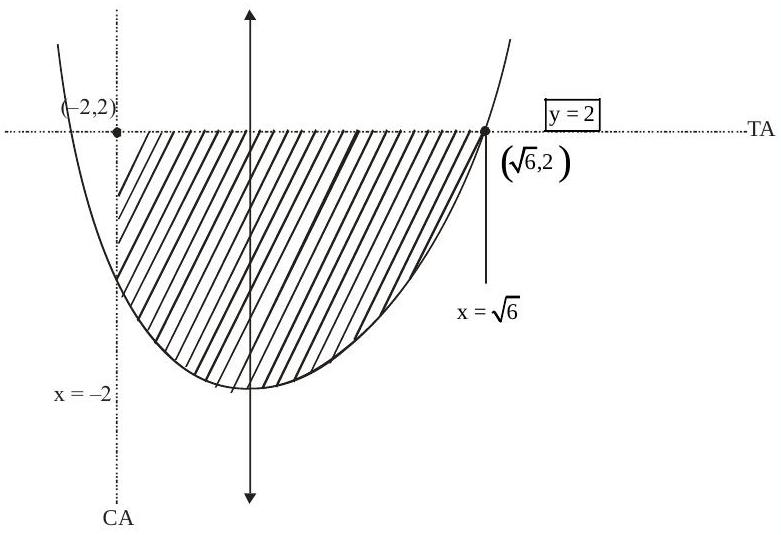
\includegraphics[max width=\textwidth, center]{2025_10_03_a6db97cda75dfa8b6db2g-06}\\
\(A=\int_{-2}^{\sqrt{6}}\left(2-\left(x^{2}-4\right)\right) d x\)\\
\(A=\int_{-2}^{\sqrt{6}}\left(6-x^{2}\right) d x=\left(6 x-\frac{x^{3}}{3}\right)_{-2}^{\sqrt{6}}\)\\
\(A=\left(6 \sqrt{6}-\frac{6 \sqrt{6}}{3}\right)-\left(-12+\frac{8}{3}\right)\)\\
\(\mathrm{A}=\frac{12 \sqrt{6}}{3}+\frac{28}{3}\)\\
\(A=4 \sqrt{6}+\frac{28}{3}\)\\
79. Let \(\vec{a}=-\hat{i}-\hat{j}+\hat{k}, \vec{a} \cdot \vec{b}=1\) and \(\vec{a} \times \vec{b}=\hat{i}-\hat{j}\). Then \(\overrightarrow{\mathrm{a}}-6 \overrightarrow{\mathrm{~b}}\) is equal to\\
(1) \(3(\hat{i}-\hat{j}-\hat{k})\)\\
(2) \(3(\hat{i}+\hat{j}+\hat{k})\)\\
(3) \(3(\hat{i}-\hat{j}+\hat{k})\)\\
(4) \(3(\hat{i}+\hat{j}-\hat{k})\)

\section*{Official Ans. by NTA (2)}
\section*{Allen Ans. (2)}
Sol. \(\quad \vec{a} \times \vec{b}=(\hat{i}-\hat{j})\)

Taking cross product with \(\vec{a}\)\\
\(\Rightarrow \quad \vec{a} \times(\vec{a} \times \vec{b})=\vec{a} \times(\hat{i}-\hat{j})\)\\
\(\Rightarrow \quad(\vec{a} \cdot \vec{b}) \vec{a}-(\vec{a} \cdot \vec{a}) \vec{b}=\hat{i}+\hat{j}+2 \hat{k}\)\\
\(\Rightarrow \quad \vec{a}-3 \vec{b}=\hat{i}+\hat{j}+2 \hat{k}\)\\
\(\Rightarrow \quad 2 \vec{a}-6 \vec{b}=2 \hat{i}+2 \hat{j}+4 \hat{k}\)\\
\(\Rightarrow \quad \vec{a}-6 \vec{b}=3 \hat{i}+3 \hat{j}+3 \hat{k}\)\\
80. The foot of perpendicular of the point \((2,0,5)\) on the line \(\frac{x+1}{2}=\frac{y-1}{5}=\frac{z+1}{-1}\) is \((\alpha, \beta, \gamma)\). Then. Which of the following is NOT correct?\\
(1) \(\frac{\alpha \beta}{\gamma}=\frac{4}{15}\)\\
(2) \(\frac{\alpha}{\beta}=-8\)\\
(3) \(\frac{\beta}{\gamma}=-5\)\\
(4) \(\frac{\gamma}{\alpha}=\frac{5}{8}\)

Official Ans. by NTA (3)\\
Allen Ans. (3)

Sol. \(\mathrm{L}: \frac{\mathrm{x}+1}{2}=\frac{\mathrm{y}-1}{5}=\frac{\mathrm{z}+1}{-1}=\lambda\) (let)\\
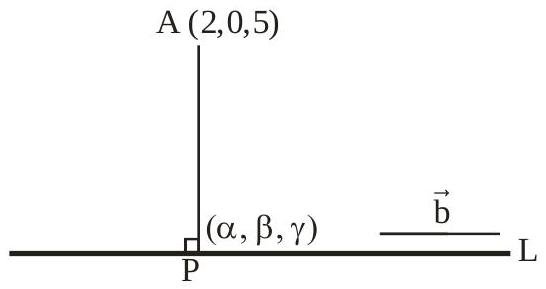
\includegraphics[max width=\textwidth, center]{2025_10_03_a6db97cda75dfa8b6db2g-07}

Let foot of perpendicular is\\
\(\mathrm{P}(2 \lambda-1,5 \lambda+1,-\lambda-1)\)\\
\(\overrightarrow{\mathrm{PA}}=(3-2 \lambda) \hat{\mathrm{i}}-(5 \lambda+1) \hat{\mathrm{j}}+(6+\lambda) \hat{\mathrm{k}}\)\\
Direction ratio of line \(\Rightarrow \vec{b}=2 \hat{i}+5 \hat{j}-\hat{k}\)

Now, \(\Rightarrow \overrightarrow{\mathrm{PA}} \cdot \overrightarrow{\mathrm{b}}=0\)\\
\(\Rightarrow 2(3-2 \lambda)-5(5 \lambda+1)-(6+\lambda)=0\)\\
\(\Rightarrow \lambda=\frac{-1}{6}\)\\
\(\mathrm{P}(2 \lambda-1,5 \lambda+1,-\lambda-1) \equiv \mathrm{P}(\alpha, \beta, \gamma)\)\\
\(\Rightarrow \alpha=2\left(-\frac{1}{6}\right)-1=-\frac{4}{3} \Rightarrow \alpha=-\frac{4}{3}\)\\
\(\Rightarrow \beta=5\left(-\frac{1}{6}\right)+1=\frac{1}{6} \Rightarrow \beta=\frac{1}{6}\)\\
\(\Rightarrow \gamma=-\lambda-1=\frac{1}{6}-1 \Rightarrow \gamma=-\frac{5}{6}\)\\
\(\therefore\) Check options

\section*{SECTION-B}
\begin{enumerate}
  \setcounter{enumi}{80}
  \item For the two positive numbers \(\mathrm{a}, \mathrm{b}\), if \(\mathrm{a}, \mathrm{b}\) and \(\frac{1}{18}\) are in a geometric progression, while \(\frac{1}{\mathrm{a}}, 10\) and \(\frac{1}{\mathrm{~b}}\) are in an arithmetic progression, then, \(16 \mathrm{a}+12 \mathrm{~b}\) is equal to \(\_\_\_\_\) .\\
Official Ans. by NTA 3\\
Allen Ans. 3
\end{enumerate}

Sol. \(\quad \mathrm{a}, \mathrm{b}, \frac{1}{18} \rightarrow \mathrm{GP}\)\\
\(\frac{\mathrm{a}}{18}=\mathrm{b}^{2}\)\\
\(\frac{1}{a}, 10, \frac{1}{b} \rightarrow \mathrm{AP}\)\\
\(\frac{1}{a}+\frac{1}{b}=20\)\\
\(\Rightarrow \mathrm{a}+\mathrm{b}=20 \mathrm{ab}\), from eq. (i); we get\\
\(\Rightarrow 18 \mathrm{~b}^{2}+\mathrm{b}=360 \mathrm{~b}^{3}\)\\
\(\Rightarrow 360 \mathrm{~b}^{2}-18 \mathrm{~b}-1=0 \quad\{\because \mathrm{~b} \neq 0\}\)\\
\(\Rightarrow \mathrm{b}=\frac{18 \pm \sqrt{324+1440}}{720}\)\\
\(\Rightarrow \mathrm{b}=\frac{18+\sqrt{1764}}{720} \quad\{\because \mathrm{~b}>0\}\)\\
\(\Rightarrow \mathrm{b}=\frac{1}{12}\)\\
\(\Rightarrow \mathrm{a}=18 \times \frac{1}{144}=\frac{1}{8}\)\\
Now, \(16 \mathrm{a}+12 \mathrm{~b}=16 \times \frac{1}{8}+12 \times \frac{1}{12}=3\)\\
82. Points \(P(-3,2), Q(9,10)\) and \(R(\alpha, 4)\) lie on a circle \(C\) with PR as its diameter. The tangents to C at the points Q and R intersect at the point S . If S lies on the line \(2 \mathrm{x}-\mathrm{ky}=1\), then k is equal to \(\_\_\_\_\) .\\
Official Ans. by NTA 3\\
Allen Ans. 3

Sol. \(\mathrm{m}_{\mathrm{PQ}} \cdot \mathrm{m}_{\mathrm{QR}}=-1\)\\
\(\Rightarrow \frac{10-2}{9+3} \times \frac{10-4}{9-\alpha}=-1 \Rightarrow \alpha=13\)\\
\(\mathrm{m}_{\mathrm{OP}} \cdot \mathrm{m}_{\mathrm{QS}}=-1 \Rightarrow \mathrm{~m}_{\mathrm{QS}}=-\frac{4}{7}\)\\
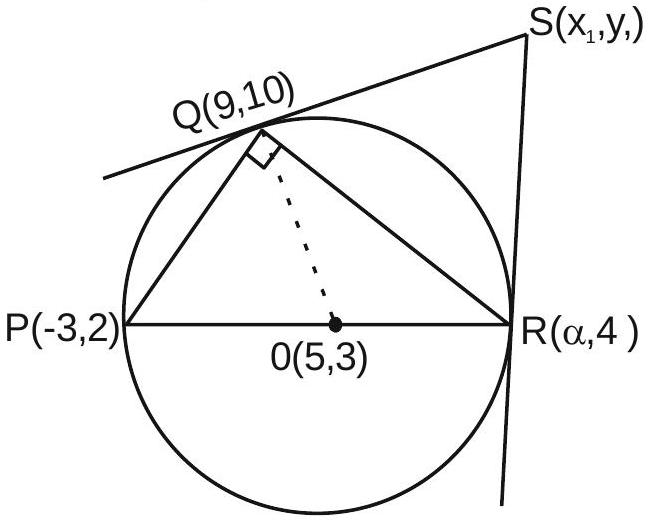
\includegraphics[max width=\textwidth, center]{2025_10_03_a6db97cda75dfa8b6db2g-08}

Equation of QS\\
\(y-10=-\frac{4}{7}(x-9)\)

\[
\Rightarrow 4 x+7 y=106
\]

\(\mathrm{m}_{0 \mathrm{R}} \cdot \mathrm{m}_{\mathrm{RS}}=-1 \Rightarrow \mathrm{~m}_{\mathrm{RS}}=-8\)\\
Equation of RS\\
\(y-4=-8(x-13)\)\\
\(\Rightarrow 8 x+y=108\)

Solving eq. (1) \& (2)\\
\(\mathrm{x}_{1}=\frac{25}{2} \mathrm{y}_{1}=8\)\\
\(\mathrm{S}\left(\mathrm{x}_{1}, \mathrm{y}_{1}\right)\) lies on \(2 \mathrm{x}-\mathrm{ky}=1\)\\
\(25-8 \mathrm{k}=1\)\\
\(\Rightarrow 8 \mathrm{k}=24\)\\
\(\Rightarrow \mathrm{k}=3\)\\
83. Let \(\mathrm{a} \in \mathrm{R}\) and let \(\alpha, \beta\) be the roots of the equation \(x^{2}+60^{\frac{1}{4}} x+a=0\). If \(\alpha^{4}+\beta^{4}=-30\), then the product of all possible values of \(a\) is \(\_\_\_\_\) .

\section*{Official Ans. by NTA 45}
\section*{Allen Ans. 45}
Sol. \(\quad x^{2}+60^{\frac{1}{4}} x+a=0 \nearrow_{\searrow \beta}^{\alpha}\)\\
\(\alpha+\beta=-60^{\frac{1}{4}} \quad \& \quad \alpha \beta=a\)\\
Given \(\alpha^{4}+\beta^{4}=-30\)\\
\(\Rightarrow\left(\alpha^{2}+\beta^{2}\right)^{2}-2 \alpha^{2} \beta^{2}=-30\)\\
\(\Rightarrow\left\{(\alpha+\beta)^{2}-2 \alpha \beta\right\}^{2}-2 \mathrm{a}^{2}=-30\)\\
\(\Rightarrow\left\{60^{\frac{1}{2}}-2 \mathrm{a}\right\}^{2}-2 \mathrm{a}^{2}=-30\)\\
\(\Rightarrow 60+4 \mathrm{a}^{2}-4 \mathrm{a} \times 60^{\frac{1}{2}}-2 \mathrm{a}^{2}=-30\)\\
\(\Rightarrow 2 \mathrm{a}^{2}-4.60^{\frac{1}{2}} \mathrm{a}+90=0\)\\
Product \(=\frac{90}{2}=45\)\\
84. Suppose Anil's mother wants to give 5 whole fruits to Anil from a basket of 7 red apples, 5 white apples and 8 oranges. If in the selected 5 fruits, at least 2 orange, at least one red apple and at least one white apple must be given, then the number of ways, Anil's mother can offer 5 fruits to Anil is \(\_\_\_\_\)\\
Official Ans. by NTA 6860\\
Allen Ans. 6860\\
Sol. 7 Red apple(RA),5 white apple(WA),8 oranges (O)\\
5 fruits to be selected (Note:- fruits taken different)\\
Possible selections :- \((2 \mathrm{O}, 1 \mathrm{RA}, 2 \mathrm{WA})\) or \((2 \mathrm{O}\),\\
2RA, 1WA) or (3O, 1RA, 1WA)\\
\(\Rightarrow{ }^{8} \mathrm{C}_{2}{ }^{7} \mathrm{C}_{1}{ }^{5} \mathrm{C}_{2}+{ }^{8} \mathrm{C}_{2}{ }^{7} \mathrm{C}_{2}{ }^{5} \mathrm{C}_{1}+{ }^{8} \mathrm{C}_{3}{ }^{7} \mathrm{C}_{1}{ }^{5} \mathrm{C}_{1}\)\\
\(\Rightarrow 1960+2940+1960\)\\
\(\Rightarrow 6860\)\\
85. If \(m\) and \(n\) respectively are the numbers of positive and negative value of \(\theta\) in the interval \([-\pi, \pi]\) that satisfy the equation \(\cos 2 \theta \cos \frac{\theta}{2}=\cos 3 \theta \cos \frac{9 \theta}{2}\), then mn is equal to \(\_\_\_\_\) .

\section*{Official Ans. by NTA 25}
Allen Ans. 25

Sol. \(\cos 2 \theta \cdot \cos \frac{\theta}{2}=\cos 3 \theta \cdot \cos \frac{9 \theta}{2}\)\\
\(\Rightarrow 2 \cos 2 \theta \cdot \cos \frac{\theta}{2}=2 \cos \frac{9 \theta}{2} \cdot \cos 3 \theta\)\\
\(\Rightarrow \cos \frac{5 \theta}{2}+\cos \frac{3 \theta}{2}=\cos \frac{15 \theta}{2}+\cos \frac{3 \theta}{2}\)\\
\(\Rightarrow \cos \frac{15 \theta}{2}=\cos \frac{5 \theta}{2}\)\\
\(\Rightarrow \frac{15 \theta}{2}=2 \mathrm{k} \pi \pm \frac{5 \theta}{2}\)\\
\(5 \theta=2 \mathrm{k} \pi\) or \(10 \theta=2 \mathrm{k} \pi\)\\
\(\theta=\frac{2 \mathrm{k} \pi}{5} \quad \theta=\frac{\mathrm{k} \pi}{5}\)\\
\(\therefore \theta=\left\{-\pi, \frac{-4 \pi}{5}, \frac{-3 \pi}{5}, \frac{-2 \pi}{5}, \frac{-\pi}{5}, 0, \frac{\pi}{5}, \frac{2 \pi}{5}, \frac{3 \pi}{5}, \frac{4 \pi}{5}, \pi\right\}\)\\
\(\mathrm{m}=5, \mathrm{n}=5\)\\
\(\therefore\) m.n \(=25\)\\
86. If \(\int_{\frac{1}{3}}^{3}\left|\log _{e} x\right| d x=\frac{m}{n} \log _{e}\left(\frac{n^{2}}{e}\right)\), where \(m\) and \(n\) are coprime natural numbers, then \(m^{2}+n^{2}-5\) is equal to \(\_\_\_\_\) .\\
Official Ans. by NTA 20

\section*{Allen Ans. 20}
Sol. \(\quad \int_{\frac{1}{3}}^{3}|\ell n x| d x=\int_{\frac{1}{3}}^{1}(-\ell n x) d x+\int_{1}^{3}(\ell n x) d x\)\\
\(=-[\mathrm{x} \ell \mathrm{nx}-\mathrm{x}]_{1 / 3}^{1}+[\mathrm{x} \ell \mathrm{nx}-\mathrm{x}]_{1}^{3}\)\\
\(=-\left[-1-\left(\frac{1}{3} \ell n \frac{1}{3}-\frac{1}{3}\right)\right]+[3 \ell n 3-3-(-1)]\)\\
\(=\left[-\frac{2}{3}-\frac{1}{3} \ell n \frac{1}{3}\right]+[3 \ell n 3-2]\)\\
\(=-\frac{4}{3}+\frac{8}{3} \ell n 3\)\\
\(=\frac{4}{3}(2 \ell n 3-1)\)\\
\(=\frac{4}{3}\left(\ln \frac{9}{\mathrm{e}}\right)\)\\
\(\therefore \mathrm{m}=4, \mathrm{n}=3\)\\
Now, \(\mathrm{m}^{2}+\mathrm{n}^{2}-5=16+9-5=20\)\\
87. The remainder when \((2023)^{2023}\) is divided by 35 is \(\_\_\_\_\) .\\
Official Ans. by NTA 7

\section*{Allen Ans. 7}
Sol. \((2023)^{2023}\)\\
\(=(2030-7)^{2023}\)\\
\(=(35 \mathrm{~K}-7)^{2023}\)\\
\(={ }^{2023} \mathrm{C}_{0}(35 \mathrm{~K})^{2023}(-7)^{0}+{ }^{2023} \mathrm{C}_{1}(35 \mathrm{~K})^{2022}(-7)+ \ldots \ldots+\ldots \ldots .+{ }^{2023} \mathrm{C}_{2023}(-7)^{2023}\)\\
\(=35 \mathrm{~N}-7^{2023}\).\\
Now, \(-7^{2023}=-7 \times 7^{2022}=-7\left(7^{2}\right)^{1011}\)\\
\(=-7(50-1)^{1011}\)\\
\(=-7\left({ }^{1011} \mathrm{C}_{0} 50^{1011}-{ }^{1011} \mathrm{C}_{1}(50)^{1010}+\ldots \ldots{ }^{1011} \mathrm{C}_{1011}\right)\)\\
\(=-7(5 \lambda-1)\)\\
\(=-35 \lambda+7\)\\
\(\therefore\) when \((2023)^{2023}\) is divided by 35 remainder is 7\\
88. If the shortest distance between the line joining the points( \(1,2,3\) ) and ( \(2,3,4\) ), and the line \(\frac{x-1}{2}=\frac{y+1}{-1}=\frac{z-2}{0}\) is \(\alpha\), then \(28 \alpha^{2}\) is equal to \(\_\_\_\_\) .

\section*{Official Ans. by NTA 18}
\section*{Allen Ans. 18}
Sol. \(\quad \vec{r}=(\hat{i}+2 \hat{j}+3 \hat{k})+\lambda(\hat{i}+\hat{j}+\hat{k}) \quad \vec{r}=\vec{a}+\lambda \vec{p}\)\\
\(\vec{r}=(+\hat{i}-\hat{j}+2 \hat{k})+\mu(2 \hat{i}-\hat{j}) \quad \vec{r}=\vec{b}+\mu \vec{q}\)\\
\(\vec{p} \times \vec{q}=\left|\begin{array}{ccc}\hat{i} & \hat{j} & \hat{k} \\ 1 & 1 & 1 \\ 2 & -1 & 0\end{array}\right|=\hat{i}+2 \hat{j}-3 \hat{k}\)\\
\(d=\left|\frac{(\vec{b}-\vec{a}) \cdot(\vec{p} \times \vec{q})}{|\vec{p} \times \vec{q}|}\right|\)\\
\(d=\left|\frac{(-3 \hat{j}-\hat{k}) \cdot(\hat{i}+2 \hat{j}-3 \hat{k})}{\sqrt{14}}\right|\)\\
\(=\left|\frac{-6+3}{\sqrt{14}}\right|=\frac{3}{\sqrt{14}}\)\\
\(\alpha=\frac{3}{\sqrt{14}}\)\\
Now, \(28 \alpha^{2}=2 / 28 \times \frac{9}{14}=18\)\\
89. \(25 \%\) of the population are smokers. A smoker has 27 times more chances to develop lung cancer then a non-smoker. A person is diagnosed with lung cancer and the probability that this person is a smoker is \(\frac{\mathrm{k}}{10}\).Then the value of k is \(\_\_\_\_\) .

\section*{Official Ans. by NTA 9}
Allen Ans. 9\\
Sol. \(\mathrm{E}_{1}\) : Smokers\\
\(\mathrm{P}\left(\mathrm{E}_{1}\right)=\frac{1}{4}\)\\
\(\mathrm{E}_{2}\) : non-smokers\\
\(\mathrm{P}\left(\mathrm{E}_{2}\right)=\frac{3}{4}\)\\
E : diagnosed with lung cancer\\
\(\mathrm{P}\left(\mathrm{E} / \mathrm{E}_{1}\right)=\frac{27}{28}\)\\
\(\mathrm{P}\left(\mathrm{E} / \mathrm{E}_{2}\right)=\frac{1}{28}\)\\
\(\mathrm{P}\left(\mathrm{E}_{1} / \mathrm{E}\right)=\frac{\mathrm{P}\left(\mathrm{E}_{1}\right) \mathrm{P}\left(\mathrm{E} / \mathrm{E}_{1}\right)}{\mathrm{P}(\mathrm{E})}\)\\
\(=\frac{\frac{1}{4} \times \frac{27}{28}}{\frac{1}{4} \times \frac{27}{28}+\frac{3}{4} \times \frac{1}{28}}=\frac{24^{9}}{30_{10}}=\frac{9}{10}\)\\
\(\mathrm{K}=9\)\\
90. A triangle is formed by X - axis, Y - axis and the line \(3 x+4 y=60\). Then the number of points \(P(a\), b)which lie strictly inside the triangle, where a is an integer and b is a multiple of a , is \(\_\_\_\_\) .

\section*{Official Ans. by NTA 31}
\section*{Allen Ans. 31}
Sol. If \(\mathrm{x}=1, \mathrm{y}=\frac{57}{4}=14.25\)\\
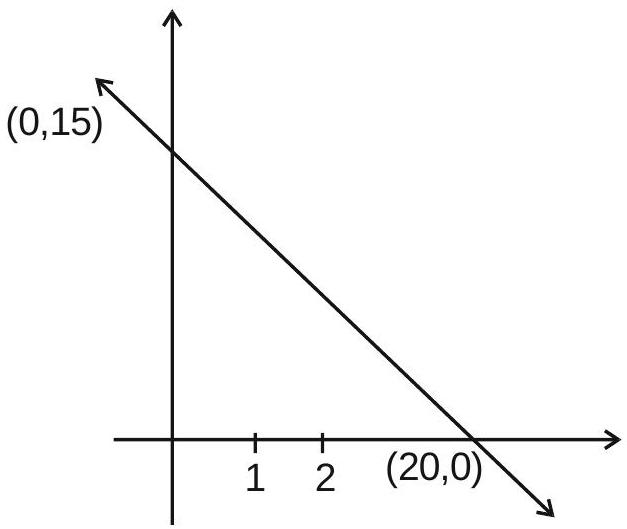
\includegraphics[max width=\textwidth, center]{2025_10_03_a6db97cda75dfa8b6db2g-10}\\
\((1,1)(1,2)-(1,14) \quad \Rightarrow 14\) pts.\\
If \(x=2, y=\frac{27}{2}=13.5\)\\
\((2,2)(2,4) \ldots .(2,12) \quad \Rightarrow 6\) pts.\\
If \(x=3, y=\frac{51}{4}=12.75\)\\
\((3,3)(3,6)-(3,12) \quad \Rightarrow 4\) pts.\\
If \(x=4, y=12\)\\
\((4,4)(4,8) \quad \Rightarrow 2\) pts.\\
If \(x=5 . y=\frac{45}{4}=11.25\)\\
\((5,5),(5,10) \quad \Rightarrow 2\) pts.\\
If \(x=6, y=\frac{21}{2}=10.5\)\\
\((6,6) \quad \Rightarrow 1 \mathrm{pt}\).\\
If \(x=7, y=\frac{39}{4}=9.75\)\\
\((7,7) \quad \Rightarrow 1\) pt.\\
If \(x=8, y=9\)\\
\((8,8) \quad \Rightarrow 1\) pt.\\
If \(x=9 y=\frac{33}{4}=8.25 \Rightarrow\) no pt.\\
Total = 31 pts.


\end{document}